% Requires:
% \usepackage{tikz}
% \usetikzlibrary{calc}

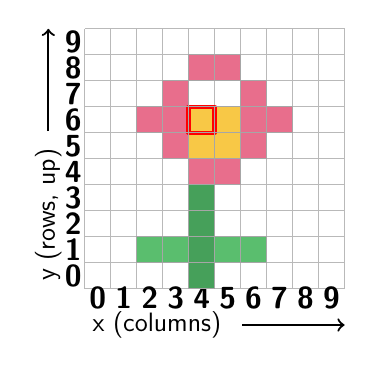
\begin{tikzpicture}[
  font={\sffamily\large},
  x=0.33cm, y=0.33cm, % pixel size
  line join=round
]
  % ---- grid size ----
  \def\W{10} % number of columns
  \def\H{10} % number of rows
  \pgfmathsetmacro{\WMinusOne}{\W - 1}
  \pgfmathsetmacro{\HMinusOne}{\H - 1}

  % ---- background ----
  \fill[white] (0,0) rectangle (\W,\H);

  % ---- draw grid ----
  \draw[step=1, gray!55] (0,0) grid (\W,\H);

  % ---- axis labels: x left->right, y bottom->top ----
  % Column indices along top: 0..W-1
  \foreach \x in {0,...,\WMinusOne} {
    \node[anchor=south, scale=1.1, font=\bfseries\sffamily, inner sep=1pt] at (\x+0.5, -0.9) {\x};
  }
  % Row indices along left, with y increasing downward:
  % Put 0 at the top row (near y=H-0.5), then 1 below it, ...
  \foreach \y in {0,...,\HMinusOne} {
    \node[anchor=west, scale=1.1, font=\bfseries\sffamily, inner sep=1pt] at (-0.9, \y+0.5) {\y};
  }

  % Optional axis titles
  \node[anchor=west, scale=0.8] at (0, -1.4) {x (columns)};
  \draw[->,line width=0.8pt] (2cm, -1.4) -s (\W,-1.4);
  \node[anchor=west, scale=0.8, rotate=90] at (-1.4, 0) {y (rows, up)};
  \draw[->,line width=0.8pt] (-1.4, 2cm) -- (-1.4, \H);

  % ---- helper: draw a pixel at (x,y) where y=0 is top row ----
  % We'll just place rectangles manually using the mapping:
  % pixel (x,y) -> rectangle from (x, H-y-1) to (x+1, H-y)

  % Colors
  \definecolor{petal}{RGB}{232,110,140}
  \definecolor{center}{RGB}{248,200,70}
  \definecolor{stem}{RGB}{70,160,90}
  \definecolor{leaf}{RGB}{90,190,110}

  % ---- flower pixels ----
  % petals (a chunky 5x5-ish flower head)


  % Petals (explicit, simpler)
  \foreach \x/\y in {
    4/1, 5/1,
    3/2, 6/2,
    2/3, 7/3,
    3/4, 6/4,
    4/5, 5/5,
    4/3, 5/3, 3/3, 6/3 % make it fuller
  }{
    \fill[petal] (\x, \H-\y-1) rectangle (\x+1, \H-\y);
  }

  % center
  \foreach \x/\y in {4/3,5/3,4/4,5/4} {
    \fill[center] (\x, \H-\y-1) rectangle (\x+1, \H-\y);
  }
  \draw[red, ultra thick] (4,6) rectangle (5,7);

  % stem
  \foreach \x/\y in {4/6,4/7,4/8,4/9} {
    \fill[stem] (\x, \H-\y-1) rectangle (\x+1, \H-\y);
  }

  % leaves
  \foreach \x/\y in {3/8,2/8,5/8,6/8} {
    \fill[leaf] (\x, \H-\y-1) rectangle (\x+1, \H-\y);
  }

  % ---- optional: outline the flower pixels slightly darker ----
  \foreach \x/\y in {
    4/1, 5/1,
    3/2, 6/2,
    2/3, 3/3, 4/3, 5/3, 6/3, 7/3,
    3/4, 4/4, 5/4, 6/4,
    4/5, 5/5,
    4/6,4/7,4/8,4/9,
    3/8,2/8,5/8,6/8
  }{
    \draw[black!35, line width=0.2pt] (\x, \H-\y-1) rectangle (\x+1, \H-\y);
  }

\end{tikzpicture}

